\chapter*{Domain}

It is impossible to perform an analysis without a thorough understanding of the context in which it is performed. At its heart, the purpose of statistics and machine learning is to glue the crystalline dimension of mathematics to a messy and unstructured world. A comprehensive understanding of the conditions of that world are required for this purpose to be successful. This ensures that the models built accurately represent what they seek to influence. Models for predictive maintenance are no exception. 

This chapter covers the domain in which a predictive maintenance process is developed. It begins with an introduction to the solar industry, its role and current state and its need for further cost reduction. It then turns its attention to predictive maintenance and provides the aims and requirements for the process. Next, the photovoltaic system is explored. Its composition, data sources and challenges in enabling predictive maintenance are discussed. Finally, a brief overview of the simulated data and model justification are provided. 



\section*{Solar Industry}

Altering the global energy mix is essential to the future evolution of civilization and possibly the survival of the species. Currently, the global energy mix is dominated by fossil fuels. Approximately, 82\% of global energy consumption remains the product of coal, natural gas and petroleum\cite{EIAOutlook2016}. A century of heavy reliance on these non-renewable fossil fuels as the central source of energy has had severe ecological and socio-economic consequences. Locally, there have been countless instances of environmental damage, such as air\cite{Tatlow2016} and groundwater\cite{Schlanger2014} contamination and oil spills\cite{OilSpills2015}. Additionally, regions rich in fossil fuels are destabilized as wealthy nations seek to guarantee future supplies\cite{Solnit2015}. Globally, the prospect of catastrophic climate change looms large, with implications including rising sea levels\cite{Davenport2015}, ocean acidification\cite{Feely2008}, crop failure\cite{Parry2004} and the economic devastation of a bursting carbon bubble\cite{Carrington2013}. 

Despite these persistent consequences, a reduction in consumption is highly unlikely. Global energy demand is projected to increase rapidly in the coming decades. As of  2012, global demand was estimated at $5.8\cdot 10^{20}$ Joules and is expected to rise by 48\% to $8.6\cdot 10^{20}$ by 2040\cite{EIAOutlook2016}. The majority of this increase is the product of higher demand for electricity, which will increase by 70\% before 2040. The majority of this new demand, roughly 87\%, is expected to come from countries in the developing world\cite{OECD2015}. Due to their economic conditions, these countries will undoubtedly utilize whichever energy source is cheapest, regardless of the consequences. 

In this context, inexpensive alternative energy production, sourced from renewable resources, is required to evade a future of socio-economic instability and ecological collapse. Fortunately, an increasing number of alternatives are being developed with the support of governments. Solar, wind, tidal, geothermal and fusion have all seen major investments over the past decade. In 2015 alone, renewable power capacity received twice the investment compared to new projects based on fossil fuels\cite{FrankfurtSchool2016}. Of these projects, wind and solar appear the most likely to become viable within the next decade\cite{OECD2014}. 

The contribution of solar energy is particularly attractive as its supplies are not limited by resource availability. At least for the next five billion years, solar energy is expected to reach the earth without interruption. Furthermore, the amount of solar radiation intercepted by the earth is several orders of magnitude higher than global energy consumption\cite{Goldemberg2000}. Given such potential, it is not surprising that the rate of installations of solar systems has increased exponentially in the past decade\cite{EPIA2014}. 

The central drivers of this growth have been continued technological development and innovative government policy. In terms of technological development, three major factors contribute to growth. First, the continued improvement of efficiency of end-use technologies. This ensures that electrical output is utilized optimally by the time it reach consumers\cite{Wilson2012}. Second, the reduction in cost and enhancement of energy storage technologies\cite{IRENA2015}. This ability is particularly important for the solar energy industry as production fluctuates based upon the availability of sunlight. Finally, and most importantly, the reduction of costs associated with technologies that convert solar energy into electricity.

In terms of reducing costs and optimizing production, the advances continue. There are frequent discoveries of novel materials which enable broader capture of solar radiation\cite{Anguita2016}. As well as developments that optimize power processing systems, ensuring that energy produced can be efficiently transfered back to the power grid\cite{Weckx2014}. These technological improvements have led to a substantial decrease in the costs associated with photovoltaic power. The average weighted utility-scale solar photovoltaic installation cost has more than halved in the last five years\cite{IRENA2016}.

However, further cost reductions are needed. The central bottleneck for greater expansion of solar power continues to be economic self-sustainability. In most markets, solar is not yet able to compete with other forms of energy generation without  government policy incentives\cite{OECD2011}. These usually come in the form of subsidies or feed-in tariffs that provide solar companies with long-term contracts for energy above market value. These are meant to provide stability as well as offset the cost of further technological development\cite{Couture2010}. However, these subsidies are reduced incrementally by design, as they are meant to serve as a temporary incentive to promote cost-saving innovation. As the subsidies are reduced, the industry is more subject to market forces and more reliant on its own ability to optimize its efficiency. The current low price of oil and coal, coupled with fickle government support for renewable energy\cite{FrankfurtSchool2016} present a difficult status quo\cite{Hals2016}. 

While technological innovation is likely to continue to reduce costs, there are avenues for further optimization given the current infrastructure. Among them are improvements in reliability, specifically in photovoltaic systems. Reliability has been a long-standing challenge\cite{Petrone2008} and a particularly important one given systems long payback periods\cite{Moore2008}. Innovation in components and manufacturing are methods for addressing reliability, but other more immediate options exist. Among them, optimized maintenance activities have the potential to dramatically reduce costs. Yet, these optimizations require predictions about the state of component health. Therefore, predictive maintenance is required.

\section*{Predictive Maintenance}

Predictive maintenance is generally defined as the process of using direct monitoring of conditions, efficiency and other indicators to determine the health and likelihood of failure of a system. These results indicate when maintenance tasks should be performed\cite{Mobley2002}. Informally, predictive maintenance is an activity geared toward indicating the degree of wear of a piece of equipment and predicting its useful life\cite{Levitt2011}. In doing so, it empowers organizations with the ability to plan and act against operational hazards. This additional time allows for corrective actions to be prepared including the ordering of parts and materials, often at lower prices, coordinating labor and scheduling downtime. In turn, this allows the business, not the environment, to dictate when service interruptions occur. 


All predictive maintenance processes attempt to address one or more of the following three generic use cases\cite{Uz2016}. First, is fault identification. Accurately identifying the source of failure of a particular system is essential to developing effective corrective countermeasures. Second, is near-term failure probability. This permits immediate operational risks to be addressed and avoided. Third, and finally, is estimation of residual lifetime. This allows both short and long-term operational risks to be taken into account. All the cases overlap and should not be treated as mutually exclusive. Yet, each requires slightly different considerations, methodology and inputs when developing a predictive maintenance process.

The preconditions for the development of a predictive maintenance process differ depending on the domain and selected use cases. Yet, there is a common core of needs including the ability to implement results, high data quality and a typical set of maintenance related sources. 

The ability implement a corrective mode of action is universal requirement. Without the ability to act, no amount of information derived from a predictive model will be of any value. After all, predictive maintenance does not, in and of itself, improve the reliability of operational systems, only maintenance activities do\cite{Levitt2011}. 

As predictive maintenance depends on condition monitoring, data sources of a suitable quality are required. Ideally, data sources should be historical, abundant, balanced, relevant and noiseless. Models that generate predictions about the future require historical data from which to derive patterns about operating conditions. The more historical information is recorded, the greater the opportunity of the model to observe the system along its lifetime. This in turn results in more accurate predictions about future health. Furthermore, the more abundant the data sources the better. As a greater number of repeated observations provides a greater certainty about the state of a system at any given time. Yet, in this context, historicity is of greater importance than abundance. It is possible to be tracking a large quantity of systems, but only for a short period of time. This would be inadequate due to a natural imbalance in the data for this type of process. Even in systems with profoundly poor reliability, healthy observations will greatly outnumber failures. Without a greater quantity of historical data, failures are even less likely to be present in the data. Therefore, a degree of balance is required in the data between the number of observed failures and healthy observations. Additionally, data sources must be relevant to the task. Data sources which offer the greatest potential for predictive power should be utilized. Domain knowledge from subject matter experts should be exploited to provide a contextually appropriate selection. These experts should also implement mechanisms that ensure data sources are as free as possible from measurement error, missing values and other forms of noise. While unavoidable in a practical setting, noise can undercut the reliability of models and introduce a greater degree of uncertainty in predictions. 

A typical set of data sources for a predictive maintenance process includes system attributes and conditions, maintenance logs and failure history\cite{Uz2016}. 

Attributes are a set of static values that define the identity of the system. This includes elements such as a system's ID, model number, date of installation, location, a list of components as well as any other technical specifications that might be relevant to its reliability. As these attributes are unlikely to change over time, they provide context which allows for the comparison of systems with one another. 

Conversely, conditions are temporal values that define the state of a system at specific points in time. These values are captured through telemetry from sensors or other periodic observations. They can include, but are not limited to, component status, yields, environmental conditions or any other time-varying data directly related to reliability. These conditions are meant to capture the evolution of a system as it ages and provide the degradation pattern leading up to failure. 

Maintenance history logs contain all service interactions with any particular system. These time stamped logs should contain any inspections, identify suspicious or replaced components and provide a listing of any corrective activities that maintenance teams performed. This data is crucial in providing context for the health of any system over time. It not only allows for the determination of the efficacy of maintenance tasks but also improves the ability to better understand the sequence of events leading up to failure.

Finally, failure history includes the time and conditions of observed breakdowns across systems. These values are usually entered manually upon system failure. An accurate and timely declaration that a machine has failed and the cause of that failure is central to the task of predictive maintenance. A generic recording of failure, without determining the cause, is not sufficient. Utmost care must be taken to ensure that the failure history records are current and complete. Delays in recording failure times detrimentally impact predictive performance. This is likely the single most important data source for a predictive maintenance process. If recorded inaccurately, it will undo the entire endeavor. 

\section*{Predictive Maintenance in Photovoltaic Inverters}

Predictive maintenance presents an opportunity for improved cost optimization in the solar industry. This section examines one area of application within the industry, namely predictive maintenance of photovoltaic inverters. First, a general picture of a typical photovoltaic system at the utility-scale is given, demonstrating the role of inverter reliability in its operation. Second, a description of the considerations when developing a predictive maintenance process in this domain are given. 


\begin{figure}[ht!]
\centering
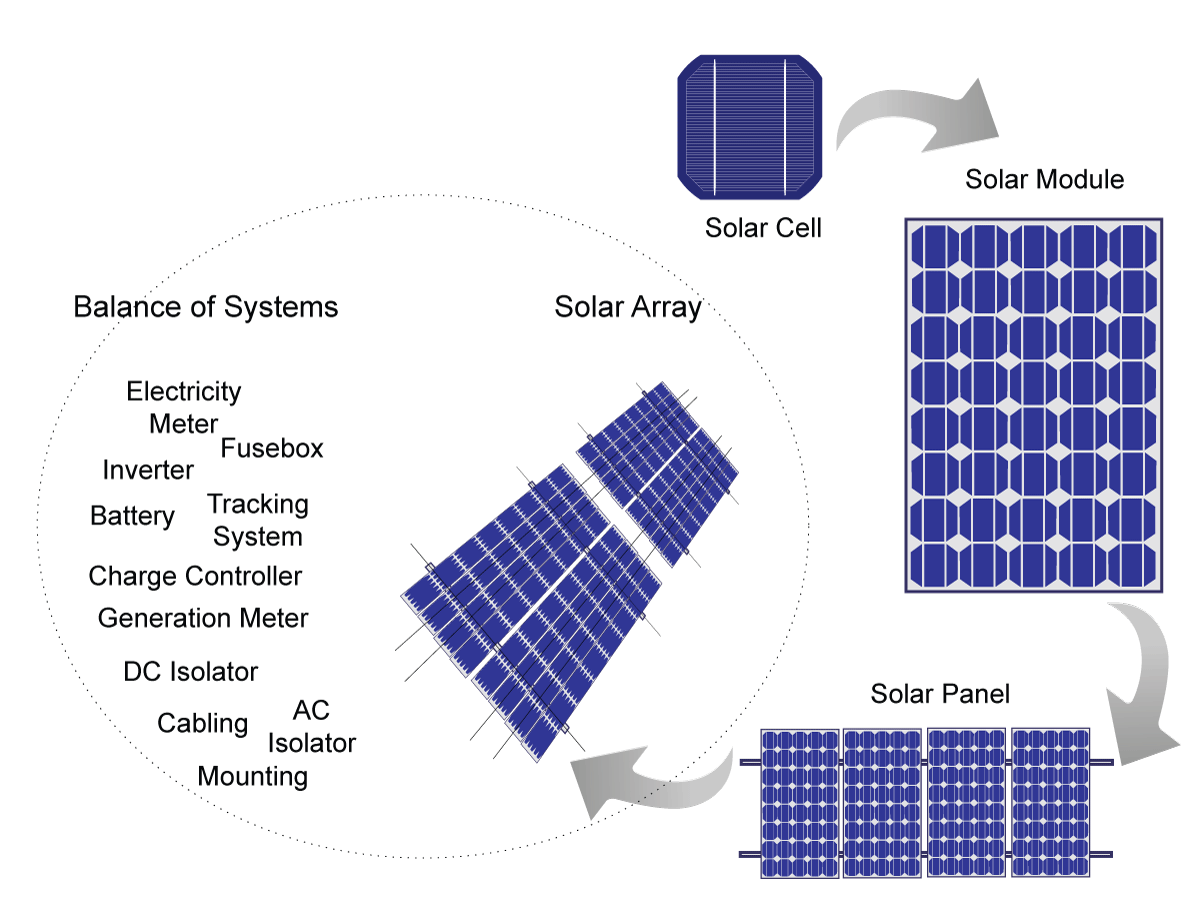
\includegraphics[width=350pt]{img/photovoltaic_system.png}
\caption{Photovoltaic System}
\label{pv_system}
\end{figure}

As can be seen in Figure~\ref{pv_system}, a typical photovoltaic system is composed of two main elements, one is a solar array and the other are balance-of-system components. 

A solar array is usually composed of individual photovoltaic cells wired in series, called a string. This is done to increase the voltage produced by individual cells. The strings are then wired in parallel to increase the current. This collection of strings is then encapsulated in a weather-resistant housing and is what we typically refer to as a solar panel. These panels are then connected to one another to form a solar array. The connection can be done in either series or in parallel depending on the desired voltage or current of the system. 

Balance-of-system (BOS) components encompass everything that is not the solar panels or array. The BOS components include the array structure, solar tracker, connectors, AC and DC wiring, over-current protections, disconnects, interconnects, charge and system controllers, maximum power point trackers, batteries, inverters and any other accessories. The purpose of the BOS components is to integrate the solar system into the utility grid.

A photovoltaic inverter is an electrical device that converts the variable DC output of the solar panels to an AC frequency allowing it to be fed to the utility grid. Of all the BOS components, the inverter has historically had the most reliability problems. A international decade-long survey of photovoltaic systems indicated that a majority of failures, 65\%, were attributed to inverters\cite{Laukamp2002}. The same research also stated there appears to be ongoing reliability improvements, as the rate of failure declined over time. Even with these improvements, recent research confirmed that inverters continued to be the most likely causes of photovoltaic system failure\cite{Golnas2013}. 

Inverter reliability is essential for ensuring steady output of a solar system. When an inverter fails, it disables all photovoltaic cells upstream of it. This makes it the single largest potential source of productivity loss in a solar system. It is for this reason, a predictive maintenance process focused on the photovoltaic inverter can serve as a valuable mechanism for optimizing operational outputs. 

Yet, there are a number of difficulties in deploying such a process within this domain. Given its role as the device connecting the solar panels to the utility grid, the inverter contains most of the intelligence in a photovoltaic system\cite{Golnas2013}. However, this intelligence is minor and narrowly focused. At any given moment, an inverter records its electrical output in kilowatt hours (kWh) and possibly provides an error code if a malfunction has been detected\cite{SMA2012}. Unfortunately, these error codes are noisy and are not always present prior to an inverter failure. Even when an error code is present, it does not uniquely define a specific cause of failure. It, instead, expresses a symptom of failure, such as current leakage, over-voltage or software error, rather than the underlying cause. Furthermore, there is a tacit acknowledgment of the lack of causality between the presence of these error codes and inverter failure. This can be seen in most dashboards of solar systems which will report a count of the number of error codes that have occurred throughout the day. Thus, a single error is not seen as particularly severe and, as stated earlier, may not even occur prior to inverter failure. 

Additionally, communication errors are relatively common with system condition data, at a rate even higher than inverter failure\cite{Golnas2013}. This results in missing values being present in historical data. As these missing values are of electrical output and error logging, it results in confusion as to whether or not the system has experienced failure or not. It also makes it impractical to use interruptions in system conditioning data as a means of detecting failure. It is an obligation of system operators to provide logs for such downtime so that this distinction can be made. However, given their frequency, and their requirement for human intervention, this often does not occur. Yet, improvements of system network connectivity are likely to resolve this problem in the near future, both in terms of on-site data collection and continuous transmission.

The lack of robust system condition data poses a challenge in developing a predictive maintenance process. At its core, the lack of condition data stems from the modularity of design in photovoltaic systems. Every additional component not directly related to generating electrical output is viewed as an operational overhead, requiring cost-benefit justifications which often do not fit into profitability planning. As a result, the inclusion of accurate sensors which track reliability indicators like temperature and humidity at the inverter level are viewed as cost prohibitive additions and generally not included. This leads to informational sparsity in photovoltaic systems and especially in inverters. 

This can be contrasted with another alternative energy source, wind, which by design does not face such problems. A wind-turbine has roughly a hundred sensors that measure everything including ambient humidity, temperature, airflow and electrical current\cite{Ciang2008}. Of course, wind-turbines are self-contained and far less modular compared to a photovoltaic system. However, other industries, such as cloud computing, that have similar modular designs do not share the same sensor deficiencies. For example, the average cloud storage server rack contains more than a hundred temperature sensors, with each server averaging three\cite{Patel2003}. The key is that the monitoring requirement of a cloud computing server rack and a solar system are comparable. Yet, there is a substantial difference in the application of sensors to create a cohesive picture of health for each unit. The cloud storage industry clearly believing that system conditioning data is worth the overhead expense. 

As the industry matures and solar power becomes independently profitable, it is likely that it too will invest more heavily in condition-based monitoring of photovoltaic inverters\cite{Feldman2014}. However, this is not yet the case. Most sensors in a solar system are at the scale of solar park as a whole, not at the scale of an inverter. Thus, temperature, humidity and solar radiance data, assuming they are recorded at all, are provided by park level sensors. With large solar parks having multiple sensors installed. This is remarkably suboptimal, as solar parks at a utility-scale can encompass a large landmass, some exceeding a hundred square kilometers. A dozen sensors scattered among that landmass will undoubtedly produce a noisy signal regarding the health of any individual inverter. There are also attempts to reduce costs of sensors by employing satellite sensor data. However, this provides even worse resolution than park-level sensor data and thus even noisier signals regarding the health of an inverter.

While the system itself may not record a substantial amount of useful data, the humans working with the systems often do. This provides contextual information which can be used in the construction of a predictive maintenance process. 

System attributes are almost always kept complete and up to date. The make, model, installation date, location and other static data are recorded. Utility-scale solar companies often have warranty contracts with manufacturers which depends on the accuracy of this data\cite{Grigoryan2010}. This often includes offers to replace faulty elements within a specific time of purchase. 

Maintenance logs and failure history are usually kept but the level of detail depends on an organization's commitment and awareness of the utility of this data. Some companies chose not to employ maintenance logs at all, instead opting for run-to-failure operations. As the name suggests, components in the system are run until they fail and are then replaced. This is an suboptimal reactive approach, and also the most expensive form of maintenance. It leads to to increased downtime and higher costs of repair parts\cite{Mobley2002}. Companies that run-to-failure will usually still store accurate failure times for these components but not always. This can result in discrepancies between failure times and a lack of system electrical output leading to confusion about exact timing of any failure\cite{Laukamp2002}. Companies that invest in some level of preventative maintenance will keep logs which include what components were inspected and what, if any, corrective measures were taken. However, the level of detail of these logs varies highly. If kept, some degree of high-level root cause is almost always included. This may be at a level that is not sufficiently discriminating such as the use of "parts and material" or "external cause" as failure categories. Some companies, especially the large ones, do provide further context for these failures, but they are usually still fairly high level, such as "control software" and "AC contactor". However, limited willingness to engage in deep-failure analysis can dampen the value of collected information\cite{Golnas2013}.

As is clear, there are some significant hurdles to overcome in the development of a predictive maintenance process within the solar energy domain. However, as the industry matures and becomes increasingly self-sustainable it will undoubtedly correct many of these imperfections. 

\section*{Simulated Data and Model Justification}

The purpose of this section is to broadly lay out the simulated data set used throughout the remainder of the text and justify the use of a Bayesian time-to-event model. 

The simulated data uses the basic designs of a real-world photovoltaic system, but lacks the faults generated by poor data management, connectivity issues and other administrative errors. The data sources of several photovoltaic companies were used as the basis for the simulated data. For the sake of exposition, the data is a simplification of reality, in that it does not cover many of the possible externalities that arise in such a system. The purpose, after all, is to demonstrate how a predictive maintenance process can be developed rather than focusing on eliminating edge-cases. Furthermore, the use of simulated data provides the ability to iteratively construct a usable model and add complexity as required. 

It contains enough similar features to allow for it to be considered a reasonably representative data set. Five-hundred inverters unevenly clustered in five solar parks are generated. Each of the five-hundred inverters is provided with an ID, a model type, and a park. One generic failure mode is used. One which occurs within the first year of operation, representing sources of infant mortality commonly found in inverters\cite{Dhere2005}. The same type of process could just as easily applied to old age wear or any other failure mode. However, given that inverters expected lifetime is a decade, this would insert added complications related to technological innovation in that period which are beyond the scope of this text.


% <!-- The other failure mode is old age wear, which peaks within ten years of operation, on average. Admittedly, this is a pessimistic choice for a time frame given improvements in inverter reliability over the preceding decade. However, it is justified in that most current solar systems will still be making use of older components. -->

% <!-- The temporal granularity of the data is daily. A predictive maintenance process could be set up on an hourly, even second basis. However, the inability to act, not to mention the time required to refit the model, makes such such narrow intervals impractical. -->

Electrical output data is provided, with both trend and seasonality removed. Furthermore, error codes are provided. Two generic error codes are generated whose combinations are related to the aforementioned failure mode. Park level data is also provided. Temperature and humidity measurements are provided at the solar park level, which are combined into an extreme weather event count. 

%<!-- All of this data is then subject to feature engineering, to extract its relevant values for the modeling process. -->

%<!-- As time-dependent data requires a trajectory in time-to-event models, this data is heavily processed to extract  -->

Finally, maintenance logs are compressed into a single activity, related to component repair or replacement within a photovoltaic inverter. It should be stressed that replacement refers to subcomponents of the inverter, like capacitors, not the inverter itself. A count of the days since the last instance of such an activity is given.

From this description, it is clear that this simulated data could be infinitely more complex. In a real-world setting, there are a greater number of failure modes, error codes and maintenance activities. However, in order to derive the essence of predictive maintenance process, this level of simplification is justified. Additionally, a real-world context is unlikely to have a greater quantity of machine condition data, only further contextual information. Thus, this additional context simply increase the dimensions of the input but does not alter the heuristic required to produce a predictive maintenance process. 

There are numerous available techniques for generating predictions of remaining lifetime. However, most of these techniques require a greater volume of condition monitoring data than is available in an average photovoltaic system. The selection of Bayesian time-to-event analysis is based on a desire to optimally use the information that is available. 

The use of time-to-event models is an acknowledgment that any system's history informs the state of any other system at similar stages of deterioration. While other methods exist that could be used for the development of a predictive maintenance process, like multiclass classification models or multiclass logit models or regression trees, none of these methods operate well in a context with a limited amount of censored data. Yet, Bayesian methods make optimal use of this small amount of available data and can be adapted to deal with censoring. Furthermore, these methods provide valuable insight into the nature and composition of breakdowns. Thus, they provide valuable information that can be used for corrective and preventive purposes outside of the predictive process.


\section*{Extended Reading}

For an understanding of international energy policy and the role that solar power plays, the OECD's World Energy Outlook is a good place to start\cite{EIAOutlook2016}. For an in-depth, but dated, introduction to predictive maintenance, the reader is directed to Mobley\cite{Mobley2002}. For a general view of constructing predictive maintenance solutions in informationally rich domains, Microsoft has assembled an excellent step-by-step guide\cite{Uz2016}. For an overview of the reliability issues specifically related to photovoltaic systems, the reader is directed to Golnas\cite{Golnas2013} and Petrone\cite{Petrone2008}. 


% Maybe add alternative methods?